%!TEX root = ../../dissertation.tex

\section{The System} % (fold)
\label{sec:the_system}

This section explains \TheName further. It presents the problems that we have faced and the respective solutions that we have found to solve them.
As expected, the main problem \TheName aims to solve is about performance. Current tools for \gls{GD} are simply too slow. We attack this problem in a number of fronts. Form diminishing the amount of data that is transferred between layers, to the management of the size of the model that is processed.

\subsection{Transferring Data} % (fold)
\label{sub:transferring_data}

One problem that we encountered on the traditional approaches is the amount of data that is transferred from the GD Tools to the module where it is processed and visualized, usually CAD's. 
%The load that is transfered heavy it was to process all that data that is serialized and deserialized at both ends of the communication channel. 
This is a bottleneck that we aimed to solve.

Our solution to this was to transfer the minimum data possible between modules of the system. To achieve this, instead of sending the whole model description, with every point information (position, color, etc.) we did something different. We send a minimum set of descriptors for each object and generate the model as late as possible within the pipeline. 

For each object we support there is a set of attributes that we need to generate, as described in Figure~\ref{fig:datalayout}. This attributes are an object type, a transformation matrix, the color of the object and a number for the scale. This is a fixed number of data that is sent between layers. This might be a problem for very simple primitives since it some times could fit in less data with the traditional approach. But it is easily compensated with more complex primitives. For instance, the data for the points to model a sphere would be much higher than the data we need for our attributes to describe it.


\begin{table}[]
\centering
\begin{tabular}{|l|l|l|l|}
\hline
\multicolumn{4}{|c|}{19 floats}                                           \\ \hline
matrix (13 floats) & color (3 floats) & type (2 floats) & scale (1 float) \\ \hline
\end{tabular}
\captionof{figure}{Data Layout}\label{fig:datalayout}
\end{table}

% subsection transferring_data (end)

\subsection{Generating Primitives} % (fold)
\label{sub:generating_primitives}

We define primitives as any model that can be modeled by one, description as described in the Section~\ref{sub:transferring_data}.

Since we use a description of the models instead of the whole information, we need to generate the primitives at some point. We do this within the GPU with shaders. More specifically geometry shaders. We support limit set of primitives, all geometric solids, that we believe are able to produce a meaningful set of different models.
Those are: Prisms, Pyramids and Spheres. Note that the prisms include Box's, Cylinders and anything in between.

With this we use simple 3D modeling parametric algorithms to generate the primitives according to the description. This allows us to have the models as late as possible. This fact helps us improve the performance of our system as explained in Section~\ref{sub:size}.

% subsection generating_primitives (end)

\subsection{Model Processing} % (fold)
\label{sub:size}

We aim to support very large models with our system. This means that sometimes, part of the model might be not visible form the current camera position. The \glspl{GPU} are able to cut out this parts of the models when they are processing the faces. This requires that the entire model is generated before it is cut out. For very large models, this process happens too late. For instance, if we have a very large model of a city. It happens that the entire city is behind the camera. The whole model is generated to be after discarded, and this is obviously not good for the performance of the system.

To work on a better solution we take advantage of the timing in which the primitives are generated and apply the Occlusion Culling technique, Section~\ref{sub:occlusion_culling}. When each description of the object is received by the \gls{GPU}, we can know if this object is currently visible form taking into account the position of the camera. With this information we can stop the generation of the object at the beginning, thus generating only the objects that are visible.

Another technique that we implement, and the constant generation of the primitives is that we can manage the Level of Detail at the generation phase.


% subsection performance (end)


\subsection{Transformation} % (fold)
\label{sub:transformation}

Since the objects are generated, we have to implement a transformation solution to generate the object correctly. We tested some options, having as a goal to minimize the number of data needed, this way diminishing the transported data.

\subsubsection{Minimum data} % (fold)
\label{ssub:minimum_data}

First we tried to implement the transformation with the minimum possible data.

Translations and scales can be trivially implemented. By centering the object at a desired point and by creating the objects with an unitary size and then multiplying by the scale, respectively. This two transformations used 3(three) floats each, 6(six) in total. 

For the rotation we implemented the axis-angle representation\cite{curtright2014compact}. This way, we only use 4(four) floats, three for the axis of rotation $\phi$, and the angle $\theta$.

We this solutions we could generate an object with the desired size, rotation and position. 

It happened that the rotation had an issue. The rotation in the axis perpendicular to $\phi$ is undefined, when $\phi$ is not parallel to any of $xyz$ axis. 
Another issue is that this solution is not cumulative. Meaning that we could not create an object and after that, apply any other transformation.

This problems made us look for another solution.

\begin{figure}[h!]
	\centering
	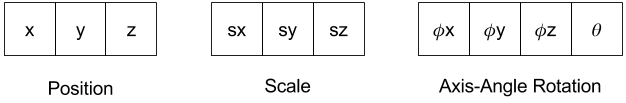
\includegraphics[width=0.75\textwidth]{images/solution/Axis-Angle_Representation.png}
	\caption{caption}
	\label{fig:axis_angle}
\end{figure}

% subsubsection minimum_data (end)

\subsubsection{Transformation Matrix} % (fold)
\label{ssub:transformation_matrix}

To solve the mentioned problems, we had to compromise on the used data. The previous solution used a total of ten floats to represent the data. 
By using a $4\times4$ matrix we would use six more floats, and could solve both issues.


\begin{figure}[h!]
	\centering
	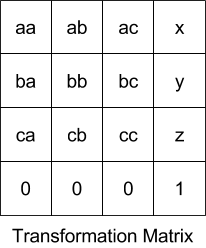
\includegraphics[width=0.25\textwidth]{images/solution/Transformation_Matrix.png}
	\caption{caption}
	\label{fig:tmatrix}
\end{figure}

(...)

% subsubsection transformation_matrix (end)



% subsection transformation (end)

\subsection{Adding Color} % (fold)
\label{sub:adding_color}

The assignment of color to the objects was a desired feature, to make \TheName more similar to the other systems. But since we want the minimum amount of data, just adding three more values to transport was not a good solution. To avoid that, we used the last line of the transformation matrix to transport the color values. Thus we could add a totally new feature without adding any more data to transport, just by better using the available space, as shown in Figure~\ref{fig:color_matrix}. This solution makes the data usage gap shorter between the option of having the transformation matrix, Section~\ref{ssub:transformation_matrix}, versus the minimum data option, Section~\ref{ssub:minimum_data}.

\begin{figure}[htbp]
	\centering
	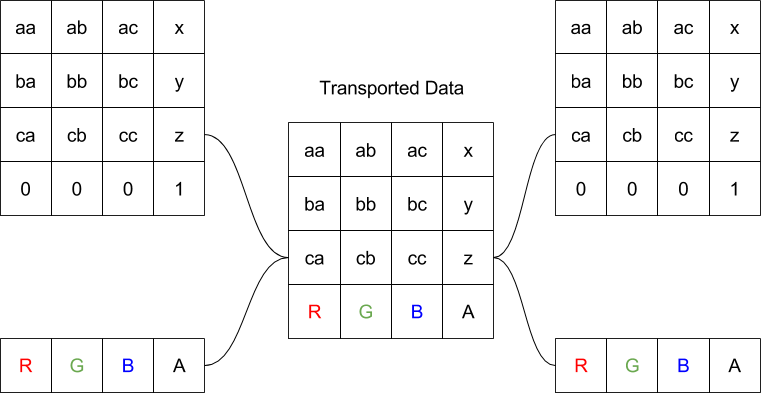
\includegraphics[width=0.95\textwidth]{images/solution/Matrix+Color.png}
	\caption{Transport of the transformation and color data}
	\label{fig:color_matrix}
\end{figure}

% subsection adding_color (end)






% section the_system (end)